\documentclass[11pt]{article}
\usepackage[margin=1in]{geometry}
\usepackage{booktabs}
\usepackage{graphicx}
\usepackage{amsmath}
\usepackage{multirow}
\usepackage{caption}
\usepackage{hyperref}
\hypersetup{hidelinks}
\sloppy
\captionsetup{font=small,labelfont=bf}
\newcommand{\rot}[1]{\begin{turn}{0}#1\end{turn}}
\usepackage{rotating}
\title{One-Day-Ahead Value-at-Risk Forecasting for SPY\\[2mm]
\large A Frozen Out-of-Sample Study of Historical Simulation, GARCH-t, HAR Quantile Regression, and Small Neural Quantile Models}
\author{Altair Li}
\date{\today}
\begin{document}
\maketitle

\section{Executive Summary}
This report studies one-day-ahead Value-at-Risk (VaR) forecasting for SPY log returns at the 1\%, 5\% and 10\% lower tails, under a strictly causal rolling-window protocol. Six model families are compared on a frozen out-of-sample period starting 2008-01-01: rolling Historical Simulation (HS), GARCH(1,1) with Student-$t$ innovations, GJR-GARCH(1,1,1)-$t$, linear (HAR-style) quantile regression, a small multi-quantile MLP, and a small GRU quantile model. Feature ablations isolate the incremental value of realized volatility (rv5), bipower variation (bv), and jump/downside-asymmetry information. All numbers in this report are regenerated by scripts from machine-readable prediction artifacts; none are hand-entered.

\section{Problem Definition}
For each forecast origin $t$ we predict the conditional return quantile $q_{\alpha,t+1}$ with $P(r_{t+1}\le q_{\alpha,t+1}\mid\mathcal{F}_t)=\alpha$ for $\alpha\in\{0.01,0.05,0.10\}$, using only information available at the end of day $t$. A violation is defined as $r_{t+1}\le \hat{q}_{\alpha,t+1}$ (VaR is the return quantile itself; lower-tail values are typically negative).

\section{Data}
Daily SPY observations with columns \texttt{log\_ret}, \texttt{rv5} (5-minute realized variance) and \texttt{bv} (bipower variation). See Appendix~\ref{sec:audit} for the machine-generated data audit.

\section{Exploratory Analysis}
See Figures~\ref{fig:overview}--\ref{fig:rvbv}. Key features: volatility clustering, heavy tails (excess kurtosis), strong persistence of log realized measures, and a positive link between negative returns and next-day volatility.

\section{Experimental Protocol}
Development period: all dates before 2008-01-01 (rolling-origin validation over 2005--2007, with a documented slight adjustment for the 1500-day window whose earliest feasible origin is late 2005). Final test: all dates from 2008-01-01. Candidate windows: 1000 and 1500 trading days only; the primary window is chosen from development evidence (see Section~\ref{sec:dev}). All models share the same forecast dates. The final configuration and data hash are frozen in \texttt{docs/FREEZE\_MANIFEST.md} before any final-test run; the gate is enforced by tests and scripts.

\section{Models}
\subsection{M0 -- Historical Simulation}
The empirical quantile of the rolling-window returns: $\hat{q}_\alpha = \hat{F}_t^{-1}(\alpha)$ over $\{r_{t-W+1},\dots,r_t\}$. Non-parametric benchmark; implicitly assumes a stationary return distribution within the window, so regime shifts are absorbed only with a lag.

\subsection{M1 -- GARCH(1,1)-Student-$t$}
Classical conditional volatility model with conditional variance
\begin{equation}
\sigma_t^2 = \omega + \alpha\,\varepsilon_{t-1}^2 + \beta\,\sigma_{t-1}^2, \qquad \varepsilon_t = \sigma_t z_t,
\end{equation}
where $z_t$ is an i.i.d.\ unit-variance standardized Student-$t$ innovation with $\nu$ degrees of freedom (variance 1, so that $\mathrm{Var}(\varepsilon_t\mid\mathcal{F}_{t-1})=\sigma_t^2$). The one-day-ahead VaR is
\begin{equation}
\mathrm{VaR}_{\alpha,t+1} = \mu + F_t^{-1}(\alpha;\nu)\,\hat\sigma_{t+1},
\end{equation}
with $F_t^{-1}(\alpha;\nu)$ the quantile of the standardized Student-$t$ (implemented via \texttt{arch.univariate.\allowbreak StudentsT}, equal to $t_\nu^{-1}(\alpha)\sqrt{(\nu-2)/\nu}$); $\mu$ is a constant mean. Parameters are re-estimated by MLE on every rolling window.

\subsection{M4 -- GJR-GARCH(1,1,1)-Student-$t$}
Adds a leverage term to the variance recursion,
\begin{equation}
\sigma_t^2 = \omega + \alpha\,\varepsilon_{t-1}^2 + \gamma\,I(\varepsilon_{t-1}<0)\,\varepsilon_{t-1}^2 + \beta\,\sigma_{t-1}^2,
\end{equation}
capturing asymmetric responses of volatility to negative shocks; VaR construction identical to M1. Serves as the downside-asymmetry robustness extension.

\subsection{M2 -- Linear / HAR Quantile Regression}
Direct conditional quantile estimation by minimizing the pinball loss,
\begin{equation}
\hat{\beta}_\tau = \arg\min_\beta \sum_t \rho_\tau\big(y_{t+1} - x_t^\top\beta\big), \qquad \rho_\tau(u) = u\big(\tau - I(u<0)\big),
\end{equation}
fit separately for $\tau \in \{0.01, 0.05, 0.10\}$ on the same feature sets as the MLP (so the linear-vs-nonlinear contrast is not confounded by information). Independent fits may cross; the crossing rate is reported.

\subsection{M3 -- Multi-Quantile MLP}
A small MLP with joint pinball loss over the three tails and a structurally non-crossing head:
\begin{equation}
q_{0.01} = z_1, \qquad q_{0.05} = z_1 + \mathrm{softplus}(z_2), \qquad q_{0.10} = q_{0.05} + \mathrm{softplus}(z_3),
\end{equation}
so that $q_{0.01}\le q_{0.05}\le q_{0.10}$ holds by construction ($\mathrm{softplus}>0$). Targets are standardized with train-only statistics inside each rolling window and the affine transform is inverted on output (Scheme B, audit fix). Training uses early stopping on the last 10\% of the window in time order; scalers are fitted on training rows only.

\subsection{M5 -- GRU Quantile}
A one-layer GRU over the last 22 daily feature vectors with the same ordered head and loss. The role is a robustness extension: it tests whether an explicit sequence representation adds value beyond the structured HAR-style features already present, not a substitute for the MLP. Parameters are deliberately kept small.

\subsection{Gaussian-GARCH diagnostic}
GARCH(1,1) with Gaussian innovations is estimated only in development as a diagnostic reference.

\section{Feature Engineering}
Information sets (identical for M2 and M3, so Linear-vs-MLP differences are attributable to the mapping rather than the inputs): \textbf{F0} returns only (lags 1/2/5/22, abs, squared); \textbf{F1} adds $\log rv5$, $\sqrt{rv5}$, 5-day and 22-day HAR aggregations of $\log rv5$; \textbf{F2} adds the same block for $bv$; \textbf{F3} adds jump proxy $\max(rv5-bv,0)$, relative jump, and a 5-day downside-shock intensity. All features are causal by construction and verified by truncation-invariance tests.

\section{Rolling Forecast Design}
A unified rolling engine controls window boundaries, feature cutoffs, preprocessing (scalers fitted on the window training rows only), model refits (daily full refit for every model), and prediction recording. Early stopping for neural models uses the last 10\% of the window in time order. All outputs share one schema (RESULTS\_SCHEMA.md) with \texttt{fit\_status} logging; failures are never silently dropped.

\section{VaR Backtesting Methodology}
Per model and tail: empirical failure rate, Kupiec unconditional coverage test, Christoffersen independence and conditional-coverage tests, mean pinball loss, quantile-crossing rate, violation clustering, Dynamic Quantile test (reported as an additional diagnostic), Diebold--Mariano tests and moving-block bootstrap for pairwise loss comparisons. Finite-sample caveats apply: the 1\% tail has very few expected violations even in a decade-long test, so coverage tests have low power and small numerical differences must not be over-read.

\section{Development / Validation Results}\label{sec:dev}
Window comparison tables: \path{outputs/development/window_selection.csv} and \path{window_selection_cells.csv}. Decision rule (predeclared, audit-fixed aggregation): per (model, feature-set, tail) cell the candidate-relative normalized loss (cell loss divided by the cell mean across the two candidates) is averaged with equal weight across all cells; per-cell winners, pairwise win counts and drop-one sensitivity are reported alongside. If the equal-weight aggregate and the raw pinball-sum aggregate disagree, the longer window is chosen conservatively for 1\% tail stability. The longer window provides more effective tail observations for the 1\% quantile (about 15 vs 10 expected violations) and hence more stable empirical quantiles, at the cost of slower regime adaptation; the short window adapts faster. The primary window selected from development evidence is \textbf{\texttt{1500}}.

\section{Frozen Out-of-Sample Results}\label{sec:oos}
All models evaluated on \texttt{2641} identical forecast dates ($\ge$ 2008-01-01). Primary seed \texttt{42}. Table~\ref{tab:metrics} reports coverage and loss statistics.

\begin{table}[ht]
\centering
\caption{Frozen out-of-sample backtesting results by model and tail.}\label{tab:metrics}
\small\begin{tabular}{lrrrrrrr}
\hline
\multicolumn{8}{l}{\textbf{Tail 1\%}}\\
\hline
\textbf{Model} & \textbf{N} & \textbf{Viol} & \textbf{Rate} & \textbf{Kupiec p} & \textbf{Ind p} & \textbf{CC p} & \textbf{Pinball}\\
HS & 2641 & 41 & 0.0155 & 0.0083 & 0.0000 & 0.0000 & 0.0006\\
GARCH-t & 2641 & 40 & 0.0151 & 0.0135 & 0.1484 & 0.0167 & 0.0004\\
LinQR & 2641 & 57 & 0.0216 & 0.0000 & 0.0411 & 0.0000 & 0.0005\\
MLP & 2641 & 87 & 0.0329 & 0.0000 & 0.0091 & 0.0000 & 0.0005\\
GJR-t & 2641 & 38 & 0.0144 & 0.0334 & 0.5766 & 0.0891 & 0.0003\\
GRU & 2641 & 85 & 0.0322 & 0.0000 & 0.0001 & 0.0000 & 0.0006\\
\hline
\multicolumn{8}{l}{\textbf{Tail 5\%}}\\
\hline
\textbf{Model} & \textbf{N} & \textbf{Viol} & \textbf{Rate} & \textbf{Kupiec p} & \textbf{Ind p} & \textbf{CC p} & \textbf{Pinball}\\
HS & 2641 & 140 & 0.0530 & 0.4819 & 0.0000 & 0.0002 & 0.0017\\
GARCH-t & 2641 & 166 & 0.0629 & 0.0035 & 0.2304 & 0.0069 & 0.0013\\
LinQR & 2641 & 161 & 0.0610 & 0.0123 & 0.0020 & 0.0004 & 0.0013\\
MLP & 2641 & 145 & 0.0549 & 0.2547 & 0.0010 & 0.0023 & 0.0013\\
GJR-t & 2641 & 167 & 0.0632 & 0.0027 & 0.3814 & 0.0075 & 0.0013\\
GRU & 2641 & 177 & 0.0670 & 0.0001 & 0.0195 & 0.0000 & 0.0015\\
\hline
\multicolumn{8}{l}{\textbf{Tail 10\%}}\\
\hline
\textbf{Model} & \textbf{N} & \textbf{Viol} & \textbf{Rate} & \textbf{Kupiec p} & \textbf{Ind p} & \textbf{CC p} & \textbf{Pinball}\\
HS & 2641 & 255 & 0.0966 & 0.5530 & 0.0006 & 0.0022 & 0.0024\\
GARCH-t & 2641 & 300 & 0.1136 & 0.0224 & 0.2361 & 0.0365 & 0.0021\\
LinQR & 2641 & 297 & 0.1125 & 0.0360 & 0.1042 & 0.0297 & 0.0021\\
MLP & 2641 & 254 & 0.0962 & 0.5100 & 0.0043 & 0.0137 & 0.0022\\
GJR-t & 2641 & 285 & 0.1079 & 0.1802 & 0.0648 & 0.0740 & 0.0020\\
GRU & 2641 & 308 & 0.1166 & 0.0054 & 0.0655 & 0.0038 & 0.0022\\
\hline
\end{tabular}
\end{table}

\section{Tail-Level Model Comparison}
See Figure~\ref{fig:tailmodel}. Rankings are tail-specific; a single universal winner is not assumed.

\section{Feature Ablations}
Table~\ref{tab:ablation} and Figure~\ref{fig:ablation}. Ablation interpretation is confined to M2/M3 across F0--F3.

\begin{table}[ht]
\centering
\caption{Feature ablation: failure rate and mean pinball by information set.}\label{tab:ablation}
\begin{tabular}{llrr}
\textbf{Model} & \textbf{Tail} & \textbf{Rate} & \textbf{Pinball}\\
M2-F0 & 1\% & 0.0170 & 0.0004\\
M2-F0 & 5\% & 0.0541 & 0.0014\\
M2-F0 & 10\% & 0.1037 & 0.0022\\
M2-F1 & 1\% & 0.0174 & 0.0004\\
M2-F1 & 5\% & 0.0557 & 0.0013\\
M2-F1 & 10\% & 0.1079 & 0.0021\\
M2-F2 & 1\% & 0.0216 & 0.0005\\
M2-F2 & 5\% & 0.0606 & 0.0013\\
M2-F2 & 10\% & 0.1121 & 0.0021\\
M2-F3 & 1\% & 0.0216 & 0.0005\\
M2-F3 & 5\% & 0.0610 & 0.0013\\
M2-F3 & 10\% & 0.1125 & 0.0021\\
M3-F0 & 1\% & 0.0360 & 0.0005\\
M3-F0 & 5\% & 0.0613 & 0.0014\\
M3-F0 & 10\% & 0.0984 & 0.0022\\
M3-F1 & 1\% & 0.0310 & 0.0004\\
M3-F1 & 5\% & 0.0568 & 0.0013\\
M3-F1 & 10\% & 0.0973 & 0.0022\\
M3-F2 & 1\% & 0.0303 & 0.0004\\
M3-F2 & 5\% & 0.0625 & 0.0013\\
M3-F2 & 10\% & 0.0981 & 0.0022\\
M3-F3 & 1\% & 0.0329 & 0.0005\\
M3-F3 & 5\% & 0.0549 & 0.0013\\
M3-F3 & 10\% & 0.0962 & 0.0022\\
\end{tabular}
\end{table}

\section{Crisis and Regime Analysis}
Figure~\ref{fig:regime} and Table~\ref{tab:regime} stratify frozen results into predefined regimes: 2008--2009 crisis, 2010--2012 elevated volatility, 2013--2014 calm, 2015--2016 stress, 2017 calm, 2018 spike. This is an explanatory analysis of frozen results, not a basis for re-optimization.

\begin{table}[ht]
\centering
\caption{Failure rate by regime (primary configuration per model).}\label{tab:regime}
\begin{tabular}{lrrrrrr}
\textbf{Regime} & GARCH-t & GJR-t & GRU & HS & LinQR & MLP\\
calm\_2013\_2014 & 0.0556 & 0.0556 & 0.0516 & 0.0020 & 0.0575 & 0.0437\\
calm\_2017 & 0.0239 & 0.0199 & 0.0239 & 0.0120 & 0.0239 & 0.0239\\
crisis\_2008\_2009 & 0.0772 & 0.0792 & 0.1366 & 0.1564 & 0.0772 & 0.0733\\
elevated\_2010\_2012 & 0.0690 & 0.0650 & 0.0544 & 0.0345 & 0.0663 & 0.0477\\
spike\_2018 & 0.0894 & 0.0894 & 0.1138 & 0.1057 & 0.0976 & 0.0976\\
stress\_2015\_2016 & 0.0595 & 0.0675 & 0.0417 & 0.0357 & 0.0496 & 0.0635\\
\end{tabular}
\end{table}

\section{Robustness}
Seed robustness for the neural models (predeclared seeds 7, 42, 2026; headline series is the primary seed 42, not an ensemble): \texttt{outputs/tables/seed\_robustness\_summary.csv}. DM and block-bootstrap pairwise comparisons: Table~\ref{tab:dm}.

\begin{table}[ht]
\centering
\caption{Pairwise loss comparisons (negative DM favors model\_a).}\label{tab:dm}
\footnotesize\begin{tabular}{llrrrrrl}
\textbf{Pair} & \textbf{Tail} & \textbf{DM} & \textbf{DM p} & \textbf{Holm p} & \textbf{Boot p} & \textbf{Favors} & \textbf{Headline}\\
M1 vs M3 & 1\% & -3.2383 & 0.0012 & 0.0048 & 0.0230 & a & H\\
M1 vs M4 & 1\% & 2.2649 & 0.0235 & 0.0705 & 0.0420 & b & H\\
M2 vs M3 & 1\% & 0.7128 & 0.4760 & 0.4760 & 0.6360 & b & H\\
M3 vs M5 & 1\% & -1.9747 & 0.0483 & 0.0966 & 0.3530 & a & H\\
M1 vs M3 & 5\% & -1.6013 & 0.1093 & 0.3279 & 0.1030 & a & H\\
M1 vs M4 & 5\% & 3.1607 & 0.0016 & 0.0063 & 0.0010 & b & H\\
M2 vs M3 & 5\% & -0.2806 & 0.7790 & 0.7790 & 0.8110 & a & H\\
M3 vs M5 & 5\% & -1.4899 & 0.1362 & 0.3279 & 0.4520 & a & H\\
M1 vs M3 & 10\% & -3.4866 & 0.0005 & 0.0015 & 0.0020 & a & H\\
M1 vs M4 & 10\% & 2.7657 & 0.0057 & 0.0114 & 0.0030 & b & H\\
M2 vs M3 & 10\% & -3.5597 & 0.0004 & 0.0015 & 0.0050 & a & H\\
M3 vs M5 & 10\% & 0.1389 & 0.8895 & 0.8895 & 0.9330 & b & H\\
\end{tabular}
\end{table}

\section{Limitations}
\begin{itemize}
\item The 1\% tail has few expected violations ($\approx$2.6 per year); coverage tests have low power.
\item Neural models are retrained daily on at most 1500 observations; capacity is deliberately small.
\item rv5/bv are daily aggregates; intraday dynamics are not modeled.
\item DM/block-bootstrap inference at extreme tails relies on asymptotic approximations; results are interpreted as indicative.
\end{itemize}

\section{Conclusion}
The conclusion is drawn from the frozen out-of-sample evidence in Section~\ref{sec:oos} and the analysis sections.

At the 1\% tail, the model with the empirical failure rate closest to the nominal level is GJR-t (0.0144 vs target 0.01); the lowest mean pinball loss is achieved by GJR-t (0.00034). Closeness of the unconditional failure frequency is not, by itself, evidence of adequate conditional VaR dynamics (see the coverage tests and the violation-clustering diagnostics below).

At the 5\% tail, the model with the empirical failure rate closest to the nominal level is HS (0.0530 vs target 0.05); the lowest mean pinball loss is achieved by GJR-t (0.00126). Closeness of the unconditional failure frequency is not, by itself, evidence of adequate conditional VaR dynamics (see the coverage tests and the violation-clustering diagnostics below).

At the 10\% tail, the model with the empirical failure rate closest to the nominal level is HS (0.0966 vs target 0.10); the lowest mean pinball loss is achieved by GJR-t (0.00204). Closeness of the unconditional failure frequency is not, by itself, evidence of adequate conditional VaR dynamics (see the coverage tests and the violation-clustering diagnostics below).

The GARCH family (GARCH-t, GJR-t) achieves the lowest mean pinball loss at all three tails. At the 1\% tail, GJR-t has the closest failure rate among the primary models (0.0144 vs 0.0151 for GARCH-t; both lie above the 1\% nominal, i.e. mildly under-conservative, and unconditional coverage rejects the nominal 1\% rate at the 5\% level for both: Kupiec p=0.0135 / 0.0334). Conditional coverage passes only for GJR-t at the 1\% tail (CC p=0.0891), while GARCH-t does not (CC p=0.0167); at the 5\% tail both fail conditional coverage (CC p=0.0069 / 0.0075). At the 10\% tail, GARCH-t fails the conditional-coverage test at the 5\% level (CC p=0.0365) whereas GJR-t does not (CC p=0.0740). At the 5\% tail HS is marginally closer to the nominal frequency (0.0530 vs 0.0629). crisis-period 5\% failure rates are 0.1564 (HS) vs 0.0772 (GARCH-t), documenting slow two-sided regime adaptation of historical simulation

The neural models do not deliver consistent absolute out-of-sample improvements over the classical baselines: the MLP is significantly worse than GARCH-t at the 1\% and 10\% tails (Holm-corrected DM p=0.0048 and 0.0015), while the 5\% difference is not statistically decisive (Holm p=0.3279); versus the linear quantile model it is significantly worse at the 10\% tail (Holm p=0.0015). The GRU is strongly under-conservative at the 1\% tail (failure rate 0.0322, far above the 1\% nominal), with the largest across-seed dispersion of the neural models. Under the pre-specified architecture family and development-only tuning, this is a valid negative result for this information set and sample; it should not be generalized to all neural VaR architectures.

Feature ablations at the 5\% tail (LinQR: RV $\rightarrow$ 4.4\%, BV$|$RV 0.1\%, F3 block -1.0\%, MLP: RV $\rightarrow$ 3.8\%, BV$|$RV -0.7\%, F3 block -1.3\%): realized volatility is the only clearly useful incremental realized-measure block; bipower variation contributes little once RV is observed; the F3 jump/downside block does not provide stable out-of-sample gains. The F3 effect is attributed to the block as a whole, not to any single component.

\section{References}
\begin{itemize}
\item Kupiec, P. (1995). Techniques for Verifying the Accuracy of Risk Measurement Models. \emph{Journal of Derivatives}, 3(2), 73--84. DOI: \url{10.3905/jod.1995.407942}
\item Christoffersen, P. (1998). Evaluating Interval Forecasts. \emph{International Economic Review}, 39(4), 841--862. DOI: \url{10.2307/2527341}
\item Engle, R. (1982). Autoregressive Conditional Heteroscedasticity with Estimates of the Variance of United Kingdom Inflation. \emph{Econometrica}, 50(4), 987--1007. DOI: \url{10.2307/1912773}
\item Bollerslev, T. (1986). Generalized Autoregressive Conditional Heteroskedasticity. \emph{Journal of Econometrics}, 31(3), 307--327. DOI: \url{10.1016/0304-4076(86)90063-1}
\item Glosten, L., Jagannathan, R., Runkle, D. (1993). On the Relation between the Expected Value and the Volatility of the Nominal Excess Return on Stocks. \emph{Journal of Finance}, 48(5), 1779--1801. DOI: \url{10.1111/j.1540-6261.1993.tb05128.x}
\item Koenker, R., Bassett, G. (1978). Regression Quantiles. \emph{Econometrica}, 46(1), 33--50. DOI: \url{10.2307/1913643}
\item Engle, R., Manganelli, S. (2004). CAViaR: Conditional Autoregressive Value at Risk by Regression Quantiles. \emph{Journal of Business \& Economic Statistics}, 22(4), 367--381. DOI: \url{10.1198/073500104000000370}
\item Andersen, T., Bollerslev, T., Diebold, F., Labys, P. (2003). Modeling and Forecasting Realized Volatility. \emph{Econometrica}, 71(2), 579--625. DOI: \url{10.1111/1468-0262.00418}
\item Barndorff-Nielsen, O., Shephard, N. (2004). Power and Bipower Variation with Stochastic Volatility and Jumps. \emph{Journal of Financial Econometrics}, 2(1), 1--37. DOI: \url{10.1093/jjfinec/nbh001}
\item Corsi, F. (2009). A Simple Approximate Long-Memory Model of Realized Volatility. \emph{Journal of Financial Econometrics}, 7(2), 174--196. DOI: \url{10.1093/jjfinec/nbp001}
\item Diebold, F., Mariano, R. (1995). Comparing Predictive Accuracy. \emph{Journal of Business \& Economic Statistics}, 13(3), 253--263. DOI: \url{10.1080/07350015.1995.10524599}
\item Koenker, R. (2005). \emph{Quantile Regression}. Cambridge University Press. DOI: \url{10.1017/CBO9780511754098}
\item Taylor, J. (2000). A Quantile Regression Neural Network Approach to Estimating the Conditional Density of Multiperiod Returns. \emph{Journal of Forecasting}, 19(4), 299--311. DOI: \url{10.1002/1099-131X(200007)19:4<299::AID-FOR775>3.0.CO;2-V}
\item Patton, A., Sheppard, K. (2015). Good Volatility, Bad Volatility: Signed Jumps and the Persistence of Volatility. \emph{Review of Economics and Statistics}, 97(3), 683--697. DOI: \url{10.1162/REST\_a\_00503}
\end{itemize}

\appendix
\section{Full Pairwise DM Matrix}\label{sec:dmappendix}
The complete 45-row pairwise Diebold--Mariano comparison matrix (exploratory; the body table shows only the predeclared headline pairs with Holm correction).
\begin{table}[ht]
\centering
\caption{Full pairwise DM matrix (all model pairs, all tails). Headline pairs are marked H.}\label{tab:dmappendix}
\footnotesize\begin{tabular}{llrrrrrl}
\textbf{Pair} & \textbf{Tail} & \textbf{DM} & \textbf{DM p} & \textbf{Holm p} & \textbf{Boot p} & \textbf{Favors} & \textbf{Headline}\\
M0 vs M1 & 1\% & 3.8448 & 0.0001 & -- & 0.2020 & b & \\
M0 vs M2 & 1\% & 2.0039 & 0.0451 & -- & 0.1230 & b & \\
M0 vs M3 & 1\% & 2.4069 & 0.0161 & -- & 0.2550 & b & \\
M0 vs M4 & 1\% & 4.0951 & 0.0000 & -- & 0.1870 & b & \\
M0 vs M5 & 1\% & -0.3931 & 0.6942 & -- & 0.8390 & a & \\
M1 vs M2 & 1\% & -1.9828 & 0.0474 & -- & 0.3570 & a & \\
M1 vs M3 & 1\% & -3.2383 & 0.0012 & 0.0048 & 0.0230 & a & H\\
M1 vs M4 & 1\% & 2.2649 & 0.0235 & 0.0705 & 0.0420 & b & H\\
M1 vs M5 & 1\% & -2.9899 & 0.0028 & -- & 0.2280 & a & \\
M2 vs M3 & 1\% & 0.7128 & 0.4760 & 0.4760 & 0.6360 & b & H\\
M2 vs M4 & 1\% & 2.2050 & 0.0275 & -- & 0.3340 & b & \\
M2 vs M5 & 1\% & -1.7255 & 0.0844 & -- & 0.2800 & a & \\
M3 vs M4 & 1\% & 3.4294 & 0.0006 & -- & 0.0220 & b & \\
M3 vs M5 & 1\% & -1.9747 & 0.0483 & 0.0966 & 0.3530 & a & H\\
M4 vs M5 & 1\% & -3.1697 & 0.0015 & -- & 0.2090 & a & \\
M0 vs M1 & 5\% & 4.5636 & 0.0000 & -- & 0.0770 & b & \\
M0 vs M2 & 5\% & 4.7905 & 0.0000 & -- & 0.0400 & b & \\
M0 vs M3 & 5\% & 3.6165 & 0.0003 & -- & 0.1170 & b & \\
M0 vs M4 & 5\% & 4.8280 & 0.0000 & -- & 0.0520 & b & \\
M0 vs M5 & 5\% & 7.1295 & 0.0000 & -- & 0.0010 & b & \\
M1 vs M2 & 5\% & -1.0079 & 0.3135 & -- & 0.4600 & a & \\
M1 vs M3 & 5\% & -1.6013 & 0.1093 & 0.3279 & 0.1030 & a & H\\
M1 vs M4 & 5\% & 3.1607 & 0.0016 & 0.0063 & 0.0010 & b & H\\
M1 vs M5 & 5\% & -2.3238 & 0.0201 & -- & 0.2890 & a & \\
M2 vs M3 & 5\% & -0.2806 & 0.7790 & 0.7790 & 0.8110 & a & H\\
M2 vs M4 & 5\% & 1.9230 & 0.0545 & -- & 0.2270 & b & \\
M2 vs M5 & 5\% & -2.2333 & 0.0255 & -- & 0.2450 & a & \\
M3 vs M4 & 5\% & 2.6703 & 0.0076 & -- & 0.0100 & b & \\
M3 vs M5 & 5\% & -1.4899 & 0.1362 & 0.3279 & 0.4520 & a & H\\
M4 vs M5 & 5\% & -2.7447 & 0.0061 & -- & 0.2220 & a & \\
M0 vs M1 & 10\% & 4.8013 & 0.0000 & -- & 0.0510 & b & \\
M0 vs M2 & 10\% & 4.9154 & 0.0000 & -- & 0.0300 & b & \\
M0 vs M3 & 10\% & 2.2617 & 0.0237 & -- & 0.1920 & b & \\
M0 vs M4 & 10\% & 5.0337 & 0.0000 & -- & 0.0290 & b & \\
M0 vs M5 & 10\% & 5.5823 & 0.0000 & -- & 0.0010 & b & \\
M1 vs M2 & 10\% & -0.1940 & 0.8462 & -- & 0.8530 & a & \\
M1 vs M3 & 10\% & -3.4866 & 0.0005 & 0.0015 & 0.0020 & a & H\\
M1 vs M4 & 10\% & 2.7657 & 0.0057 & 0.0114 & 0.0030 & b & H\\
M1 vs M5 & 10\% & -2.3423 & 0.0192 & -- & 0.2750 & a & \\
M2 vs M3 & 10\% & -3.5597 & 0.0004 & 0.0015 & 0.0050 & a & H\\
M2 vs M4 & 10\% & 1.0913 & 0.2751 & -- & 0.3070 & b & \\
M2 vs M5 & 10\% & -2.6403 & 0.0083 & -- & 0.1940 & a & \\
M3 vs M4 & 10\% & 4.3462 & 0.0000 & -- & 0.0010 & b & \\
M3 vs M5 & 10\% & 0.1389 & 0.8895 & 0.8895 & 0.9330 & b & H\\
M4 vs M5 & 10\% & -2.7877 & 0.0053 & -- & 0.2060 & a & \\
\end{tabular}
\end{table}

\section{Machine-Generated Data Audit}\label{sec:audit}
\url{docs/DATA\_AUDIT.md} (generated by \texttt{scripts/audit\_data.py}).

\section{Artifacts}
All prediction panels: \path{../outputs/runs/230b3e9702b1-09a350fe/predictions/*.parquet} with sidecar manifests; metric tables: \path{../outputs/runs/230b3e9702b1-09a350fe/tables/*.csv}; figures: \path{../outputs/runs/230b3e9702b1-09a350fe/figures/*.png}. Freeze manifest: \texttt{docs/FREEZE\_MANIFEST.md}.

\begin{figure}[ht]
\centering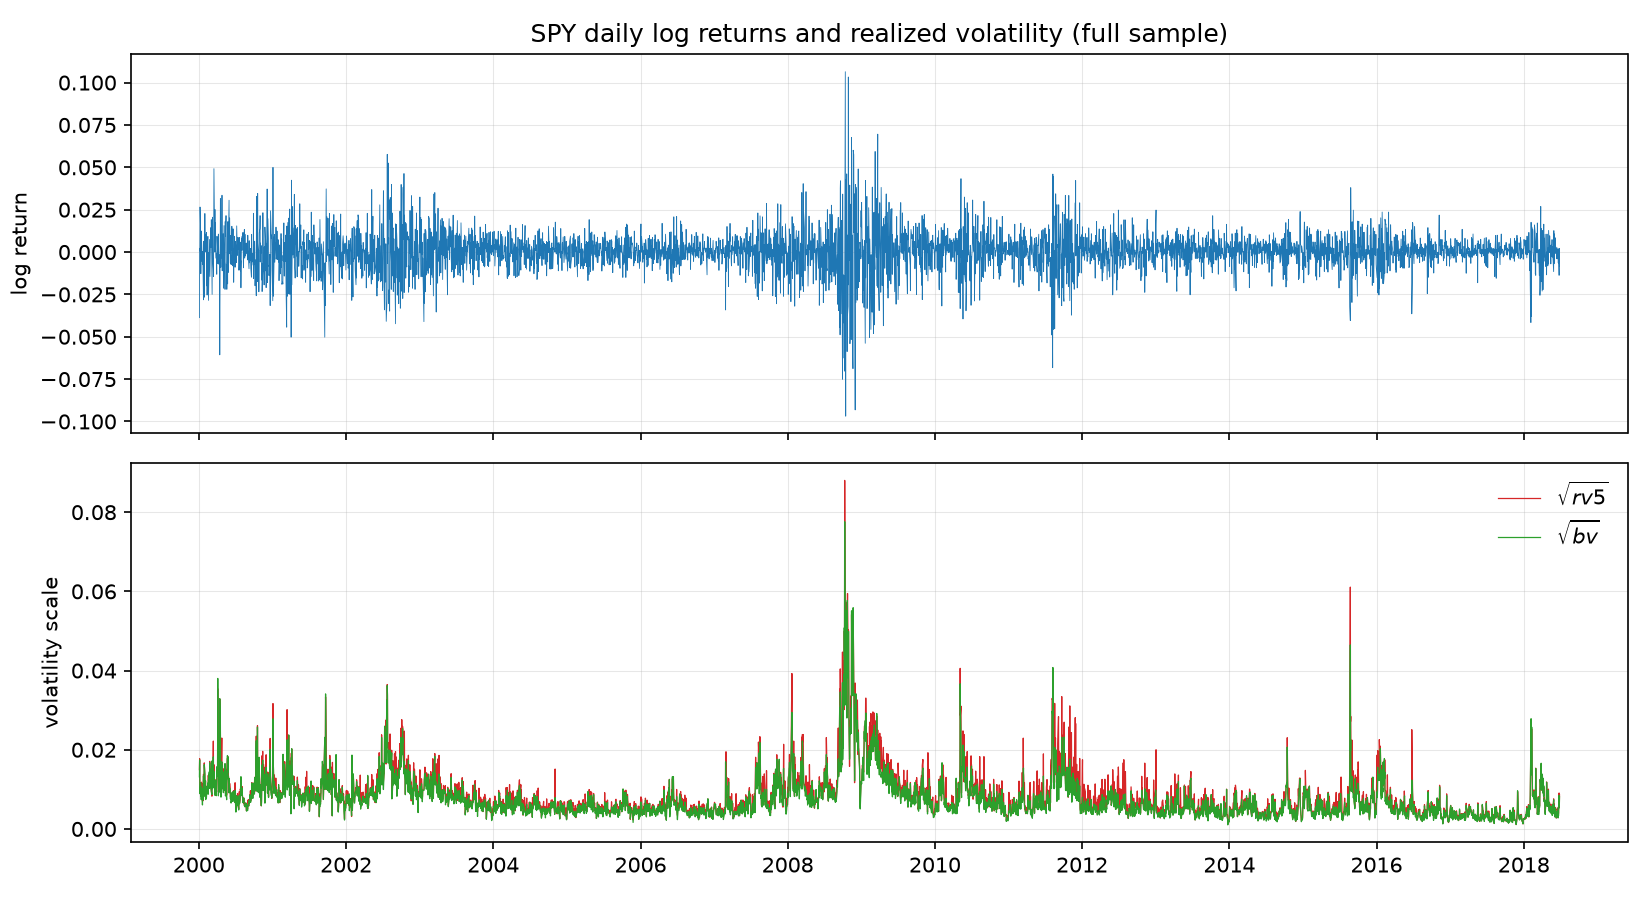
\includegraphics[width=\textwidth]{../outputs/runs/230b3e9702b1-09a350fe/figures/fig01_overview.png}
\caption{SPY log returns and volatility scale, full sample.}\label{fig:overview}
\end{figure}
\begin{figure}[ht]
\centering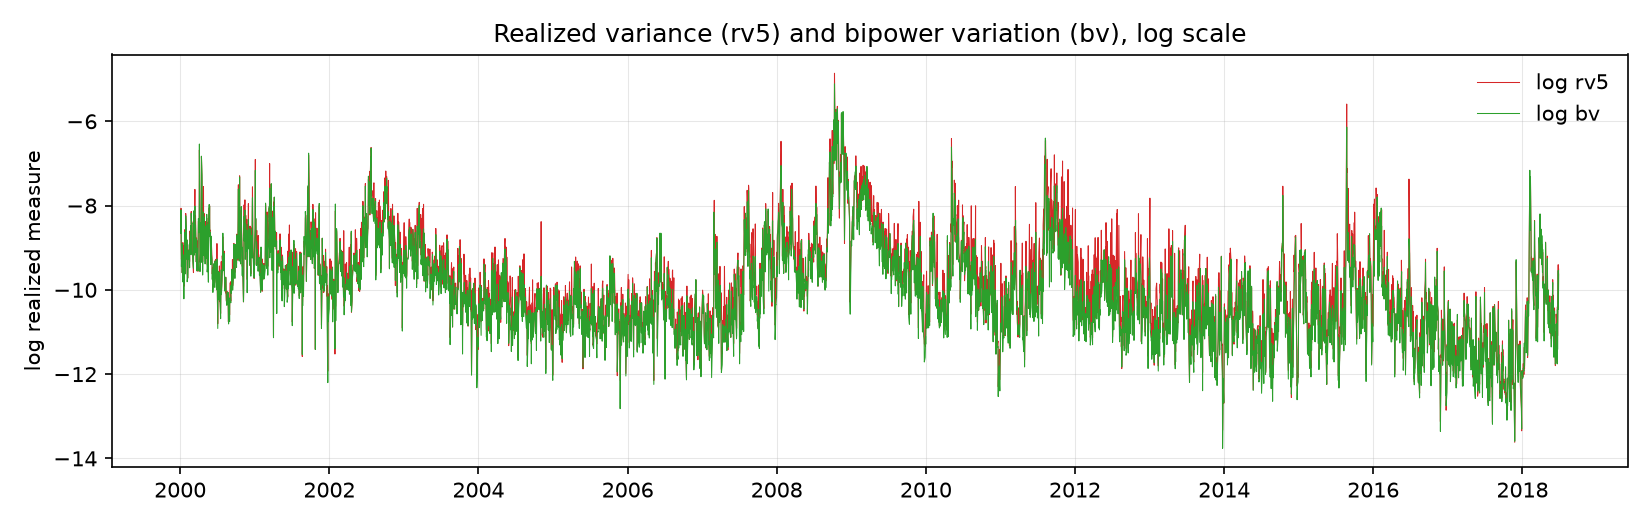
\includegraphics[width=\textwidth]{../outputs/runs/230b3e9702b1-09a350fe/figures/fig02_rv_bv.png}
\caption{Realized variance and bipower variation (log scale).}\label{fig:rvbv}
\end{figure}
\begin{figure}[ht]
\centering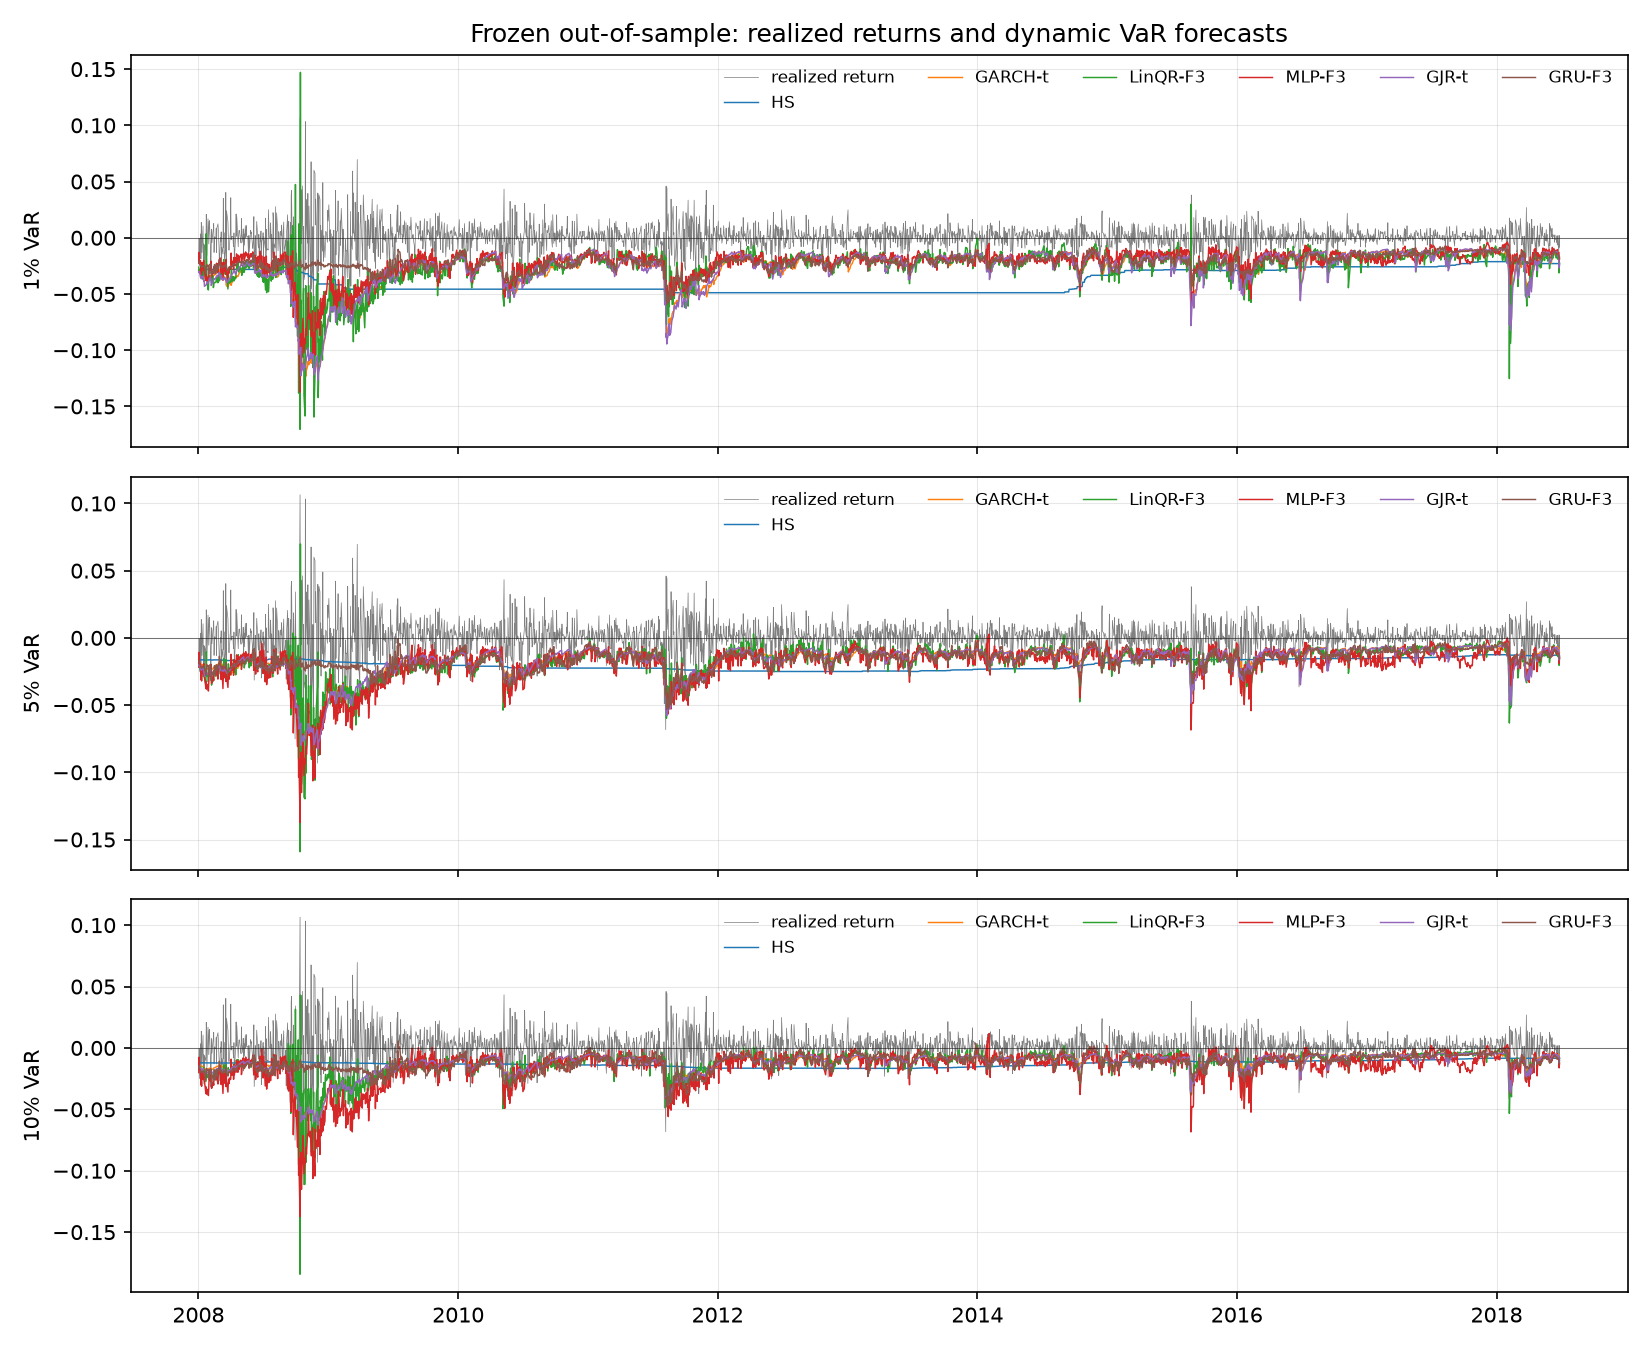
\includegraphics[width=\textwidth]{../outputs/runs/230b3e9702b1-09a350fe/figures/fig03_var_curves.png}
\caption{Frozen out-of-sample realized returns with dynamic VaR forecasts.}
\end{figure}
\begin{figure}[ht]
\centering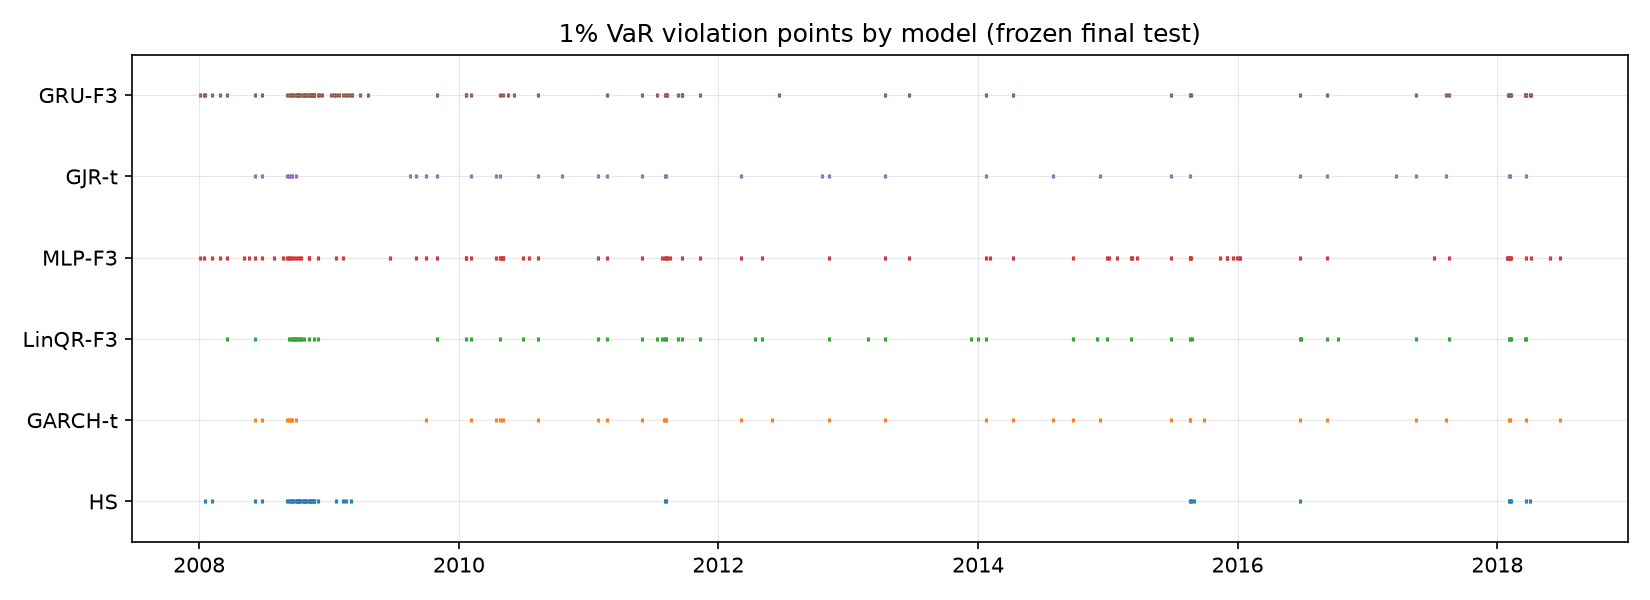
\includegraphics[width=\textwidth]{../outputs/runs/230b3e9702b1-09a350fe/figures/fig04_violations.png}
\caption{1\% VaR violation points by model.}
\end{figure}
\begin{figure}[ht]
\centering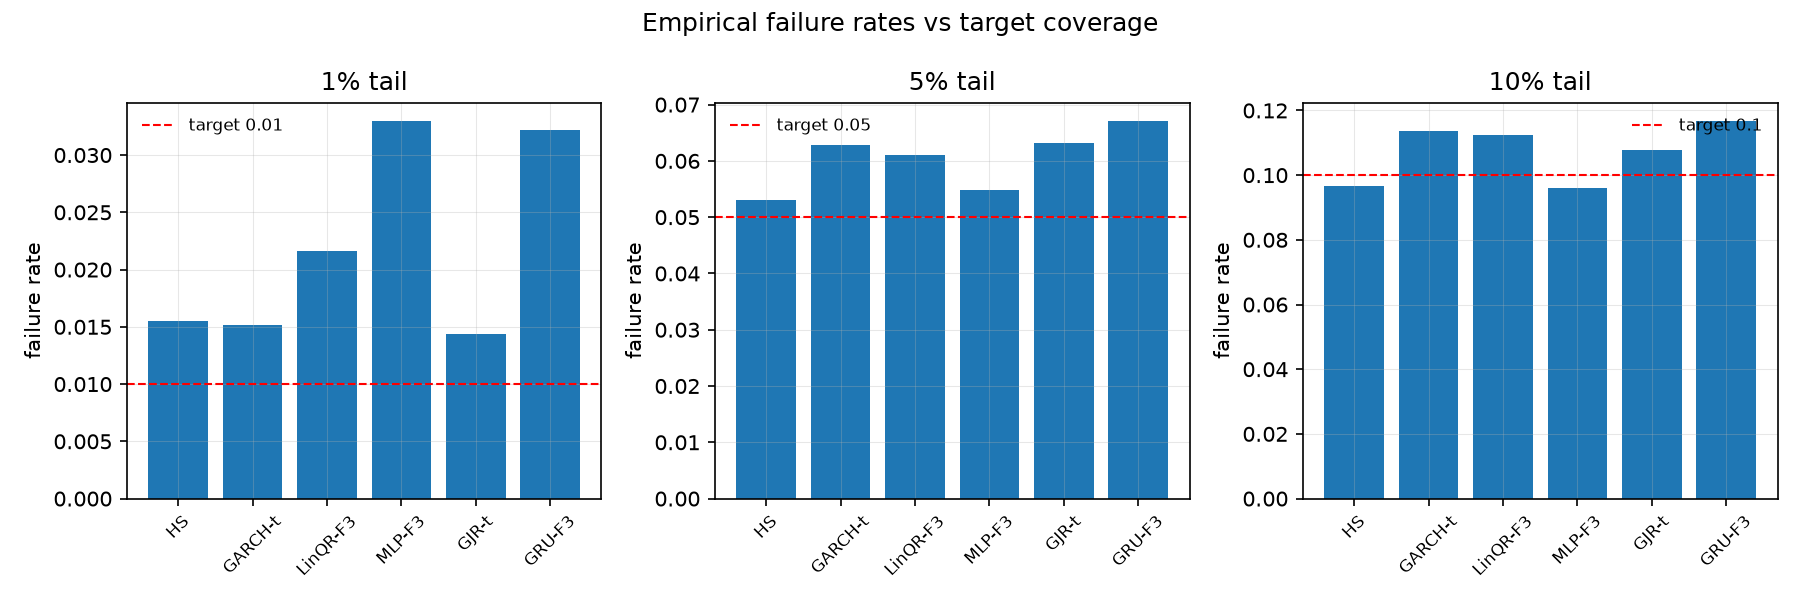
\includegraphics[width=0.85\textwidth]{../outputs/runs/230b3e9702b1-09a350fe/figures/fig05_failure_rates.png}
\caption{Empirical failure rates vs target coverage.}
\end{figure}
\begin{figure}[ht]
\centering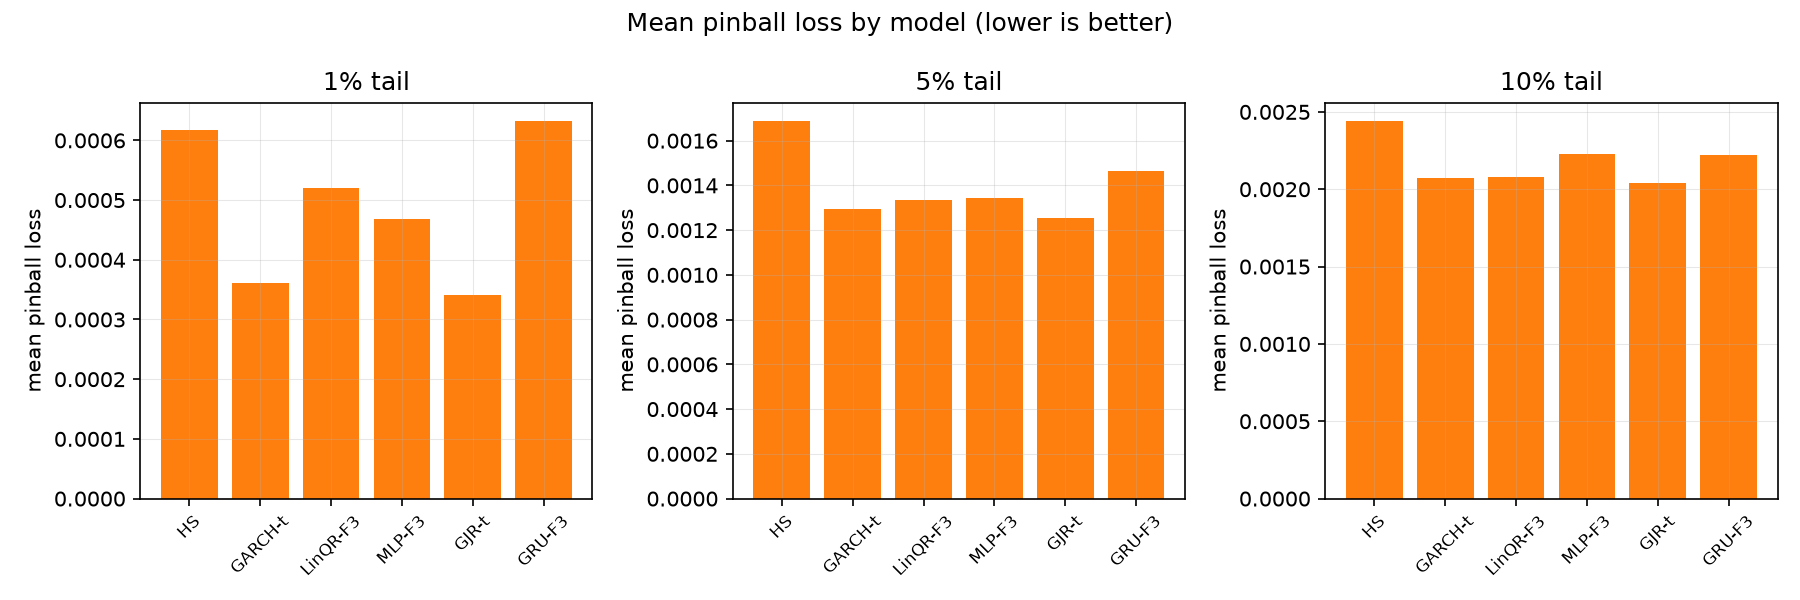
\includegraphics[width=0.85\textwidth]{../outputs/runs/230b3e9702b1-09a350fe/figures/fig06_pinball.png}
\caption{Mean pinball loss by model and tail.}
\end{figure}
\begin{figure}[ht]
\centering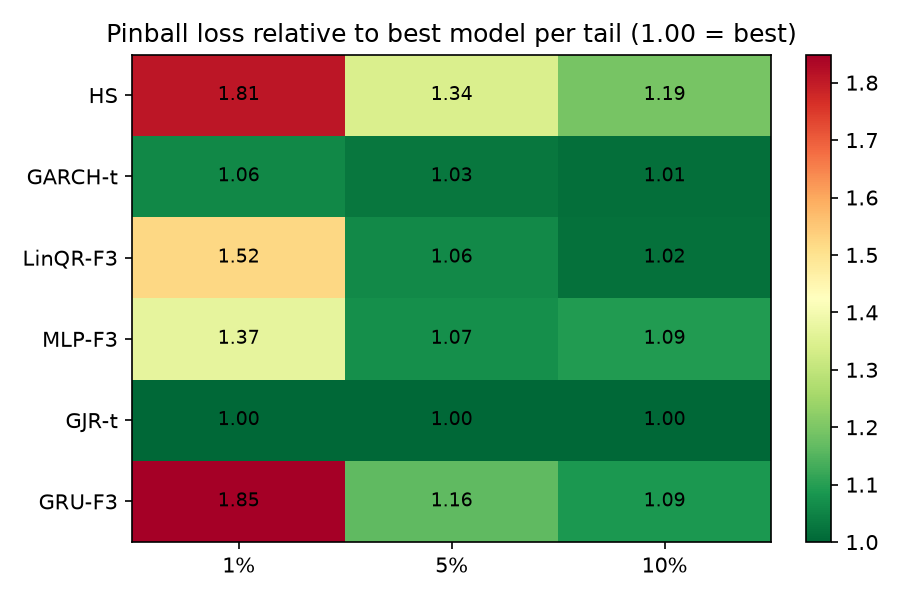
\includegraphics[width=0.6\textwidth]{../outputs/runs/230b3e9702b1-09a350fe/figures/fig07_tail_model.png}
\caption{Pinball loss relative to best model per tail.}\label{fig:tailmodel}
\end{figure}
\begin{figure}[ht]
\centering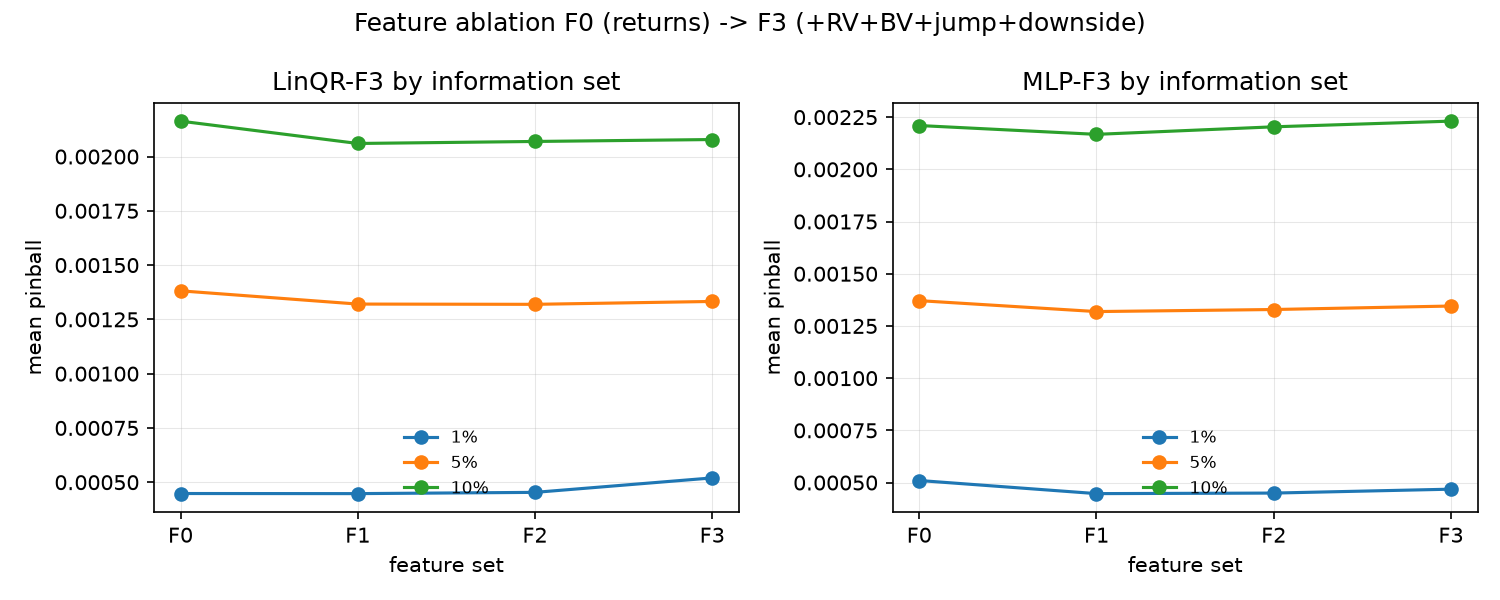
\includegraphics[width=0.8\textwidth]{../outputs/runs/230b3e9702b1-09a350fe/figures/fig08_ablation.png}
\caption{Feature ablation F0--F3 for linear quantile regression and MLP.}\label{fig:ablation}
\end{figure}
\begin{figure}[ht]
\centering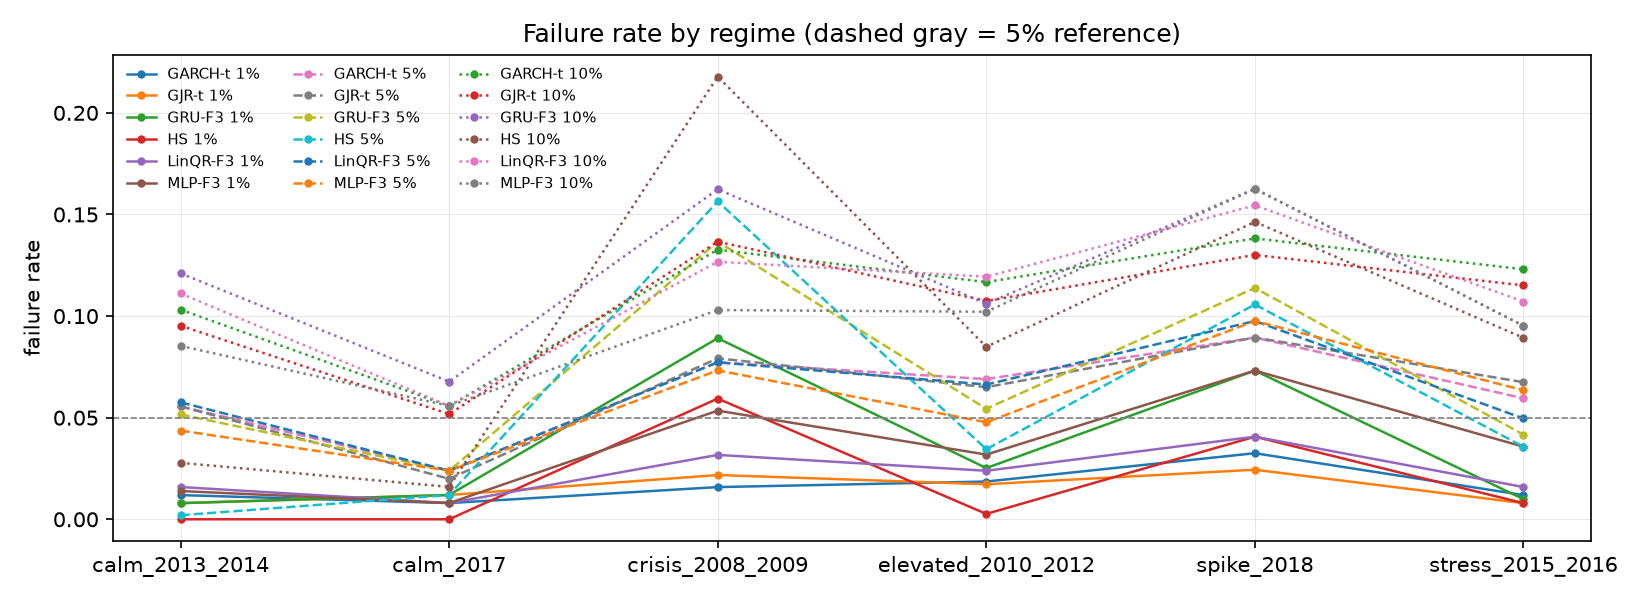
\includegraphics[width=\textwidth]{../outputs/runs/230b3e9702b1-09a350fe/figures/fig09_regime.png}
\caption{Failure rate by regime.}\label{fig:regime}
\end{figure}
\begin{figure}[ht]
\centering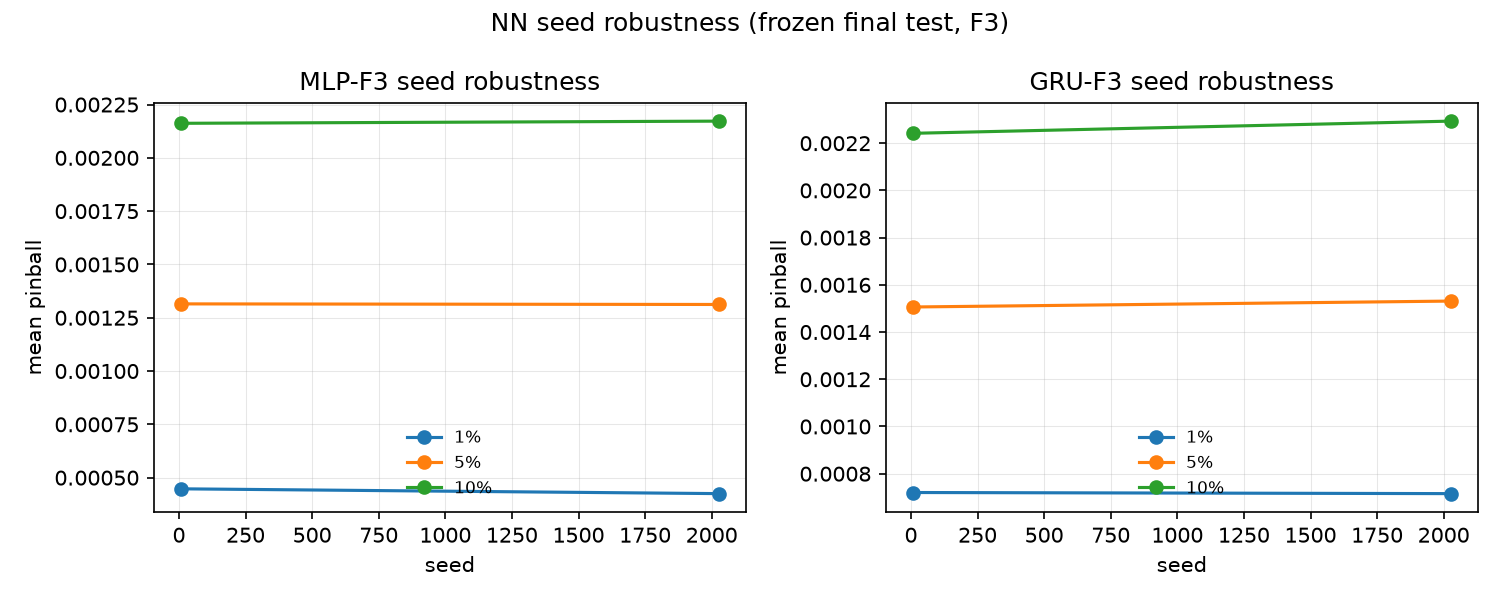
\includegraphics[width=0.8\textwidth]{../outputs/runs/230b3e9702b1-09a350fe/figures/fig10_seed_robustness.png}
\caption{Neural seed robustness.}
\end{figure}

\end{document}
